\chapter{Bayes minimum risk}\label{ch:5}

\begin{remark}{Outline}
In this chapter, we introduce the Bayes minimum risk algorithm in Section~\ref{sec:5:bmr}. Then, in 
Section~\ref{sec:5:prob}, we discuss the impact of calibrating the probabilities in the model. 
Finally, in Section~\ref{sec:5:experiments}, we compare the results of the proposed 
algorithm, against state-of-the-art methods, using the five real-world cost-sensitive databases.
\end{remark}


\section{Bayes minimum risk model}
\label{sec:5:bmr}

As decribed in Section \ref{sec:2:cs}, state-of-the-art example dependent techniques, only 
introduce the cost by modifying the training set. In \citep{CorreaBahnsen2013,CorreaBahnsen2014}, 
we proposed a cost-sensitive model called Bayes minimum risk classifier ($BMR$).  

As defined in \citep{Ghosh2006}, the BMR classifier is a decision model based on
quantifying tradeoffs between various decisions using probabilities and the costs that accompany 
such decisions. This is done in a way that for each example the expected losses are minimized. In  
what follows, we consider the probability estimates $\hat p_i$ as known, regardless of the algorithm 
used to calculate them.  The risk that accompanies each decision is calculated using the cost matrix 
as described in \tablename{ \ref{tab:2:cost_matrix}}. In the specific framework of binary 
classification, the risk of predicting the example $i$ as negative is 
\begin{equation}
  R(c_i=0|\mathbf{x}_i)=C_{TN_i}(1-\hat p_i)+C_{FN_i} \cdot \hat p_i, 
\end{equation}
and
\begin{equation}
  R(c_i=1|\mathbf{x}_i)=C_{TP_i} \cdot \hat p_i + C_{FP_i}(1- \hat p_i), 
\end{equation}
is the risk when predicting the example as positive, where $\hat p_i$ is the estimated positive 
probability for example $i$. Subsequently, if 
\begin{equation}
  R(c_i=0|\mathbf{x}_i) \le R(c_i=1|\mathbf{x}_i), 
\end{equation}
then  the example $i$ is classified as negative. This means that the risk associated with the 
decision $c_i$ is lower than the risk associated with classifying it as positive. 

\begin{remark}{Characteristics of probability estimates}
When using the output of a binary classifier as a basis for decision making, there is a 
need for a probability that not only separates well between positive and negative examples, but that 
also assesses the real probability of the event \citep{cohen2004}.
\end{remark}


\section{Calibration of probabilities}
\label{sec:5:prob}

In this section we discussed a measure for evaluating how well calibrated are a set of 
pobabilities. Furthermore, two methods for calibrating probabilities are explained. First, the 
method proposed in \citep{Elkan2001} to adjust the probabilities based on the   difference in bad 
rates  between the training and testing datasets.  Then, the method proposed in 
\cite{Hernandez-Orallo2012}, in which calibrated probabilities are extracted after modifying the ROC 
curve using the ROC convex hull methodology, is described.
  
  
\subsection{Brier score}
\todo{ask Djamila, should this be in background}

Traditional evaluation measures of binary classification problems, such as Accuracy and 
$F_1Score$, provide a way to analyze the performance of a model. However, when using the classifier 
output as a basis for decision making, there is a need of a measure that takes into account not only 
the misclassification of a classifier $\mathbf{c}$, but also the quality of the estimated 
probability $\mathbf{\hat p}$ \citep{cohen2004}. The most appropriate  is the Brier score 
\citep{brier1950}. The Brier score is one of a class of so-called proper scores which are used in 
evaluating the subjective probability assessment of forecasters \citep{DeGroot1983}. The Brier score 
is the average squared difference between the forecasters estimated probability of and the true 
label:
\begin{equation}
  BS(f(\mathcal{S})) = \frac{1}{N} \sum_{i=1}^{N} (\hat p_i - y_i)^2.
\end{equation}
The main justification of this score, is based on decision theoretic considerations, in the sense 
that, a forecaster should pay a price proportional to the confidence with which it asserts its 
decision.


\subsection{Calibration due to a change in base rates}

One of the reasons why a probability may not be calibrated is because the algorithm is trained using 
a dataset with a different base (or positive) rate than the one on the evaluation dataset.  This is 
something common in machine learning since using under-sampling or over-sampling is a typical method 
to solve problems such as class imbalance and cost sensitivity \citep{Hulse2007}.
  
In order to solve this and find probabilities that are calibrated, in \citep{Elkan2001} a formula  
that corrects the probabilities based on the difference of the base rates is proposed.  The 
objective is using $\hat p$ which was estimated using a population with base rate $\pi_1$,
to find $\hat p'$ for the real population which has a base rate $\pi_1'$. A solution for $\hat p'$ 
is given as follows:
\begin{equation}
  \hat p'=\pi_1' \frac{\hat p - \hat p \pi_1}{\pi_1- \pi_1 \hat p +\pi_1' \hat p - \pi_1 \pi_1'}.
\end{equation}

% Nevertheless, a strong assumption is made by taking: $P'(x|j=1)=P(x|j=1)$} and 
% \mbox{$P'(x|j=0)=P(x|j=0)$}, meaning that there
%   is no change in the example probability within the positive and negative
%   subpopulations density functions.
  
\subsection{Calibrated using the ROC convex hull}

In order to illustrate the ROC convex hull approach proposed in \citep{Hernandez-Orallo2012},
let us consider the set of probabilities given in \figurename{~\ref{tab:5:example_prob}}.
Their corresponding  ROC curve of that set of probabilities is shown in 
\figurename{~\ref{fig:5:ROC_1}}.  It can be seen that this set of probabilities is not calibrated, 
since at 0.1 there is a positive example  followed by 2 negative examples. That inconsistency is 
represented in the ROC curve as a non convex segment  over the curve.
  
\begin{figure}[!t]
\hskip 0.5cm
\hbox{
  \vtop{
    \hbox{
      \subfloat[Set of probabilities and their respective class label]{
   \footnotesize
	\begin{tabular}{cc}
	\hline
	Probability & Label\\
	\hline
	0.0&	0\\
	0.1&	1\\
	0.2&	0\\
	0.3&	0\\
	0.4&	1\\
	0.5&	0\\
	0.6&	1\\
	0.7&	1\\
	0.8&	0\\
	0.9&	1\\
	1.0&	1\\
	\hline
	\end{tabular}\label{tab:5:example_prob}
      }
    }
  }\hskip 0.5cm
  \vtop{\vskip -2.5cm
    \subfloat[ROC curve of the set of probabilities]{
      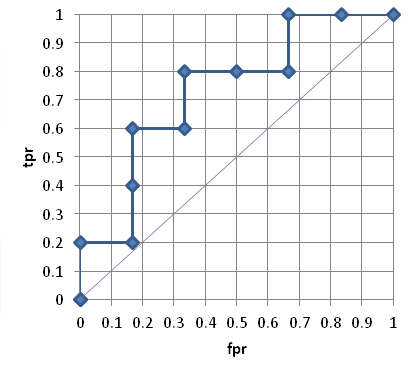
\includegraphics[scale=0.5]{ch5_fig2}\label{fig:5:ROC_1}
    }%
  }%
}
\vskip 1.5cm

\hbox{ 
  \vtop{ \vskip 0.5cm
    \hbox{
      \subfloat[Convex hull of the ROC curve]{
	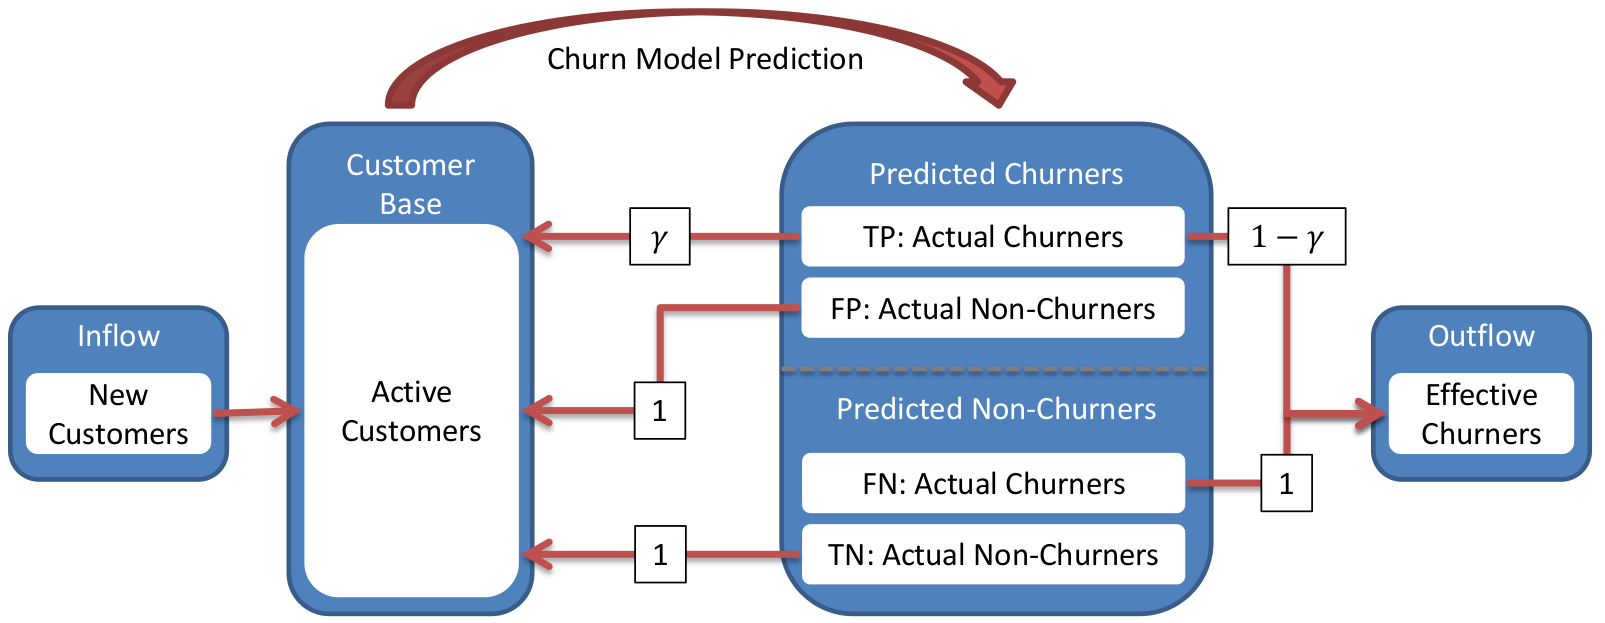
\includegraphics[scale=0.5]{ch5_fig1}\label{fig:5:ROC_2}
      }
    }
  }\hskip 1cm
  \vtop{ \vskip -1cm
    \subfloat[Calibrated probabilities]{
   \footnotesize
	\begin{tabular}{cc}
	\hline
	Prob & Cal Prob\\
	\hline
	0.0&	0\\
	0.1&	0.333\\
	0.2&	0.333\\
	0.3&	0.333\\
	0.4&	0.5\\
	0.5&	0.5\\
	0.6&	0.666\\
	0.7&	0.666\\
	0.8&	0.666\\
	0.9&	1\\
	1.0&	1\\
	\hline
	\end{tabular}\label{fig:5:cal_prob} 
    }
  }
}
\caption{Estimation of calibrated probabilities using the ROC convex hull.}\label{fig:5:rocch}
\end{figure}

In order to obtain a set of calibrated probabilities, first the ROC curve must be modified in 
order to be convex. The way to do that, is to find the convex \mbox{hull 
\citep{Hernandez-Orallo2012}}, in order to obtain the minimal convex set containing the different 
points of the ROC curve. In \figurename{~\ref{fig:5:ROC_2}}, the convex hull algorithm is applied 
to the previously evaluated ROC curve. It is shown that the new curve is convex, and includes all 
the points of the previous ROC curve.

Now that there is a new convex ROC curve or ROCCH, the calibrated probabilities can be extracted 
as shown in  \figurename{~\ref{fig:5:cal_prob}}. The procedure to extract the new probabilities is 
to first group the probabilities according to the points in the ROCCH curve, and then make the 
calibrated  probabilities be the slope of the ROCCH for each group.
  
   
\section{Experiments}
\label{sec:5:experiments}
\todo{experiments}